\documentclass{article}

\usepackage[spanish]{babel}
\usepackage{fontenc}
\usepackage[utf8]{inputenc}
\usepackage{hyperref}
\usepackage{graphicx}
\usepackage{amsmath}
\usepackage{amsfonts}
\usepackage{amssymb}
\usepackage{amsthm}
\usepackage[left=30pt,right=40pt,top=40pt,bottom=60pt]{geometry}

\author{NyKi}
\date{Enero 2025-}

% Entornos
\theoremstyle{definition}
\newtheorem{theorem}{Teorema}
\newtheorem{prop}{Proposición}
\newtheorem{cor}{Corolario}
\newtheorem{axiom}{Axioma}
\newtheorem{define}{Definición}
\newtheorem{note}{Nota}
\newtheorem{ejem}{Ejemplo}

\DeclareMathOperator{\trace}{tr}

% Conjuntos
\newcommand{\reales}{\mathbb{R}}
\newcommand{\naturales}{\mathbb{N}}
\newcommand{\racionales}{\mathbb{Q}}
\newcommand{\cinfinito}{\mathcal{C}^{\infty}}
\newcommand{\claseck}[1]{\mathcal{C}^{#1}}


\begin{document}

Por comodidad, asumiremos que $\naturales$ (el conjunto de los números naturales) empiezan en el $1$ (es decir, no contienen al $0$).
Antes de empezar voy a dar unas definiciones y resultados de análisis que se usan aquí.

\begin{define}
	Una aplicación $f:U\subseteq\reales^n \rightarrow \reales^m$ con $n,m$ enteros mayores a 0 y $U$ abierto no vacío se denomina \textbf{de clase $\claseck{k}$} si admite parciales hasta el orden $k \in \naturales$ y estas son continuas.
\end{define}
\begin{define}
	Una aplicación $f:U\subseteq\reales^n \rightarrow \reales^m$ con $n,m$ enteros mayores a 0 y $U$ abierto no vacío se denomina \textbf{de clase $\cinfinito$} si admite parciales de todos los órdenes y estas son continuas.
\end{define}
Es un resultado de un curso de análisis que una aplicación $\cinfinito$ definida sobre un dominio abierto es diferenciable. Otro nombre para las funciones $\cinfinito$ es suave.
\begin{define}
	Una aplicación $f:I \rightarrow J$ con $I,J$ intervalos abiertos de números reales se dice $difeomorfismo$ si es biyectiva, derivable y su inversa también es derivable.
\end{define}
De la definición se puede ver que un difeomorfismo es también un homeomorfismo.

\section{Curvas parametrizadas}


\begin{define}
	Decimos que una aplicación $\alpha: I \rightarrow \reales^2$ (con $I$ un intervalo abierto de $\reales$) de clase $\claseck{k}$ es una \textbf{curva parametrizada k-diferenciable} (o paramétrica). El conjunto $\alpha(I)$ se denomina \textbf{traza} de la curva y lo denotamos mediante $\trace(\alpha)$.
\end{define}
En general simplemente las llamaremos curvas diferenciables, excluyendo la clase de la función, y asumiendo que admiten todas las derivadas que necesitamos (y estas son continuas). Es viable también definir las curvas como aplicaciones $\cinfinito$, pero le quita un poco de generalidad a la teoría. En esta definición nos hemos restringido a intervalos abiertos de la recta real. Es posible considerar intervalos cerrados, pero nos tenemos que asegurar que la función en los extremos se pueda ``extender'':
\begin{define}
	Decimos que una aplicación $\alpha: I \rightarrow \reales^2$ (con $I$ un intervalo cerrado de $\reales$) de clase $\cinfinito$ es una \textbf{curva parametrizada diferenciable} si existe una curva paramétrica diferenciable $\beta: I^* \rightarrow \reales^2$ definida sobre un intervalo abierto $I^*$ que contiene a $I$ tal que $\beta  \big|_I = \alpha$ y $\beta^{(k)}  \big|_I = \alpha^{(k)}$ para todo $k \in \naturales$.
\end{define}
Aunque esta definición presenta algún que otro problema, como veremos al hablar de curvas cerradas. Cuando hablemos de curvas definidas sobre un intervalo, simplemente asumiremos que es abierto.
Veamos algunos ejemplos de curvas parametrizadas.
%Simplemente considerar aplicaciones $\cinfinito$ sobre intervalos cerrados sin que se puedan extender puede llegar a problemas:
\begin{ejem}[De curvas]
\begin{enumerate}
	\item
	La curva $\alpha (t) = (t, t^2)$ definida en $\reales$ es una parábola. \\ 
	\item 
	La circunferencia unidad centrada en $0$ $\alpha(t) = (\cos t, \sin t)$ definida en $[0, 2*\pi]$. \\ 
	\item
	La curva $\alpha(t) = (\cos 2t, \sin 2t)$ definida en $\reales$ tiene como traza la misma circunferencia que en el ejemplo anterior.
	\item
	La curva $\alpha(t) = (\frac{1-t^2}{1+t^2}, \frac{2t}{1+t^2})$ definida en $\reales$ tiene como traza la misma circunferencia excluyendo el punto $(-1, 0)$.
	\item
	$\alpha(t) = (\frac{a\cos t}{1 + \sin^2 t}, \frac{a\sin t \cos t}{1 + \sin^2 t})$ definida en $\reales$ es la lemniscata de Bernoulli.
\end{enumerate}
\end{ejem}

Las curvas son objetos geométricos. Por tanto es raro (o a lo mejor contraintuitivo) representarlas mediante funciones reales. Pero esto se hace por una buena razón: queremos usar métodos diferenciales para estudiar la geometría de la traza de las curvas. Dada por ejemplo la circuferencia clásica $(x-a)^2 + (y-b)^2 = r^2$ hemos visto que existen muchas curvas paramétricas diferenciables tales que su traza sea igual a ella, y por tanto a un conjunto de $\reales^2$ le pueden corresponder muchas curvas. El objetivo es encontrar o crear cantidades independientes de la curva que usemos para describir una traza, es decir buscar \textbf{invariantes geométricos}.\\ 
Para esto hacemos un intento de formalizar curvas que tienen la misma traza:

\begin{define}
	Dada una curva diferenciable $\alpha: I \rightarrow \reales$ y un difeomorfismo $f: J \rightarrow I$ con $I,J$ intervalos abiertos decimos que la composición $\beta = \alpha \circ f : J \rightarrow \reales$ es una \textbf{reparametrización} de la curva $\alpha$, y $f$ es el \textbf{parámetro}.
\end{define}

Notamos que bajo esta definición es posible que al reparametrizar una curva obtengamos una que sea de clase menor que la original. Llevaremos un poco de cuidado con ello cuando lo necesitemos. También será importante tener en cuenta la orientación la orientación del difeomorfismo:

\begin{define}
	Dado $f: J \rightarrow I$ difeomorfismo entonces o $f'(x) < 0\ \forall x \in J$ o $f'(x) > 0\ \forall x \in J$. En el primer caso se dice que f \textbf{invierte} la orientación y en el segundo que la \textbf{conserva}.
\end{define}

El hecho sobre el signo de la derivada del difeomorfismo es un hecho conocido del análisis. La orientación de una curva no es un hecho absoluto sino que es relativo (es decir, no podemos decir que una curva tiene una cierta orientación si no la comparamos con alguna otra). Ahora podemos demostrar:

\begin{prop}\label{prop_curvas_traza}
	Si $\alpha: I \rightarrow \reales$ es una curva diferenciable y $\beta: J \rightarrow \reales$ es una reparametrización de $\alpha$ entonces $\trace (\alpha) = \trace (\beta)$.
\end{prop}

La implicación conversa (trazas iguales implican que son reparametrizaciones) la demostraremos después. Para ello vamos a tener que introducir los conceptos que vamos a usar para estudiar las curvas localmente. Primero, veamos un ejemplo:

\begin{ejem}[Curva suave que no lo parece]
	La curva $\alpha: [-1, 1] \rightarrow \reales^{2}$ dada por:
	\begin{equation}
		\alpha = \left\lbrace \begin{array}{lr}
			(-t^4, t^4 )& \ \text{para}\ t \in [-1, 0]\\
			(t^4, t^4 )& \ \text{para}\ t \in (0, 1]\\
		\end{array} \right.
	\end{equation}
	tiene la siguiente gráfica:
	\begin{center}
		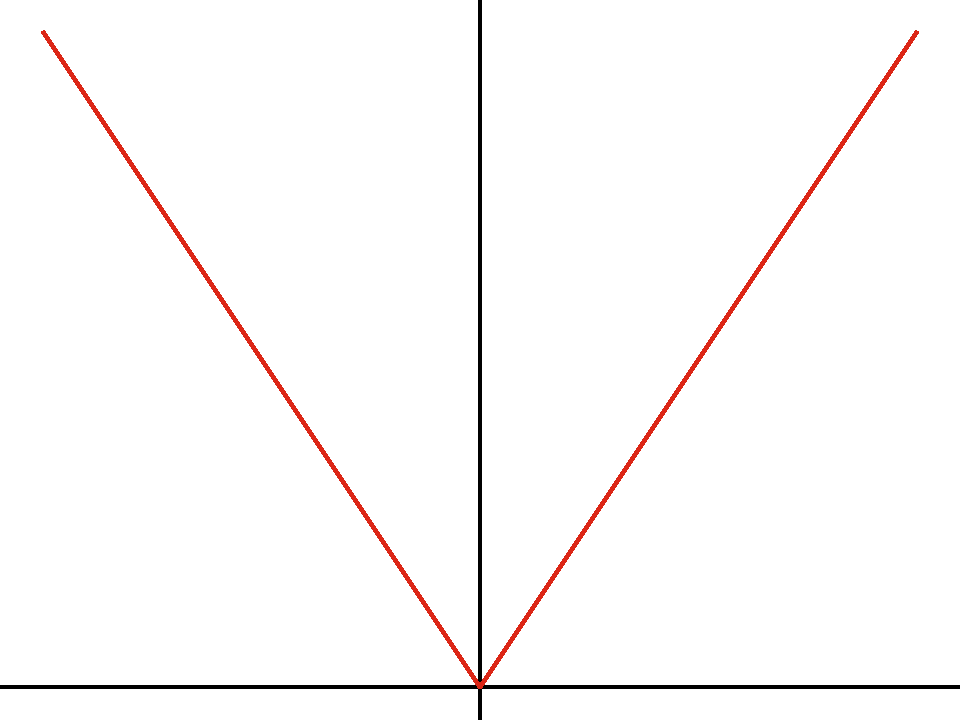
\includegraphics[scale=0.4]{gfx/ej1_2.pdf}
	\end{center}
	Se puede comprobar que la curva es de clase $\claseck{2}$, pero la gráfica es la misma que la de la función valor absoluto, que no es diferenciable en $x=0$. En este ``pico'' la derivada de la curva es $(0, 0)$.
\end{ejem}
La situación de este ejemplo es algo que intuitivamente queremos evitar: contradice la noción de ser \textit{suave}. La causa de este problema es que en este punto no existe una recta tangente bien definida, ya que el vector derivada es nulo. Solo nos interesa trabajar con curvas en las que esto no pase:

\begin{define}
	Una curva diferenciable $\alpha: I \rightarrow \reales^{n}$ se dice \textbf{regular} si $\alpha(t) \neq 0$ para todo $t \in I$. 
\end{define}

Una curva regular es tal que todo punto de la traza tiene por lo menos una recta tangente. Esto no significa que necesariamente sea única:

\begin{ejem}[Lemniscata de Bernoulli]

\end{ejem}

Ahora nuestro objetivo es establecer un parámetro que nos proporcione una forma ``natural'' de trabajar con una curva. De esta manera a una traza resultante de alguna curva regular le asignaremos una curva de alguna manera canónica (aunque esto no sea del todo posible, se ve más abajo).

\begin{define}
	Dada una curva diferenciable $\alpha: I \rightarrow \reales^{n}$ definimos su \textbf{longitud} desde $a$ hasta $b$ con $a\leq b \in I$ como la cantidad $\int_a^b |\alpha' (t)| dt$, y la denotaremos como $L_{a}^{b} (\alpha)$. 
\end{define}

Aquí damos una definición de longitud. Se podría demostrar que el producto escalar sobre $\reales^{n}$ da lugar (usando la definición de integral de Riemann) a está fórmula, pero nosotros no demostraremos esto.\\ 
Esta noción proporciona una invariante de una curva:

\begin{prop}
	Sea $\alpha: I \rightarrow \reales^{n}$ una curva diferenciable y $\beta: J \rightarrow \reales^{n}$ una reparametrización de $\alpha$. Si $t_0, t_1 \in I$, $s_0, s_1 \in J$ son tales que $\alpha(t_0) = \beta(s_0)$ y $\alpha(t_1) = \beta(s_1)$ entonces $L_{t_0}^{t_1} (\alpha) = L_{s_0}^{s_1} (\beta)$.
\end{prop}

\begin{define}
	Una curva diferenciable $\alpha: I \rightarrow \reales^{n}$ se dice \textbf{parametrizada por la longitud del arco} o \textbf{natural} si se tiene $|\alpha' (t)| = 1$ en todo $I$.
\end{define}

Esto nos dará para cada traza una curva ideal:

\begin{prop}	
	Para toda curva diferenciable regular existe una reparametrización por la longitud del arco.
\end{prop}

\begin{define}
	La aplicación $s$ de la demostración anterior se denomina \textbf{parámetro longitud de arco}.
\end{define}

La última proposición demuestra que siempre es posible encontrar una reparametrización de una curva regular de manera que el vector derivada sea siempre unitario. Es posible encontrar más de una para cada curva:

\begin{ejem}
	La circunferencia $\alpha(t) = (\cos t, \sin t)$ definida en todo $\reales$ está parametrizada por la longitud del arco (como se puede comprobar). La curva $\beta(t) = (\cos (-t), \sin (-t))$ definida en $\reales$ también es natural y es una reparametrización de $\alpha$ mediante $f(t) = -t$. 
\end{ejem}

Así, hablaremos de \textit{una} parametrización por arco. Ahora podemos demostrar el converso de la proposición \eqref{prop_curvas_traza} para cierta familia de curvas:

\begin{cor}
	Si dos curvas regulares tienen la misma traza entonces una curva es una reparametrización de la otra y conversamente.
\end{cor}

Finalmente en esta sección hablamos de curvas cerradas. Intuitivamente, una curva cerrada es una curva $\alpha$ definida sobre un intervalo cerrado $[a, b]$ con $a,b \in \reales$ y $a < b$ tal que $\alpha(a) = \alpha(b)$. Esta definición no es perfecta:

\begin{ejem}
	
\end{ejem}

En vista de esto, es necesario añadir algo más a la definición:

\begin{define}
	Una curva k-diferenciable $\alpha: I \rightarrow \reales^{n}$ con $I = [a, b]$ intervalo cerrado con $a < b$ ambos reales se dice \textbf{cerrada} si se cumple $\alpha^{(m)}(a) = \alpha^{(m)}(b)$ para todo $m \in \{1, \dots, k\}$.
\end{define}

Solo demostraremos la siguiente proposición:

\begin{prop}
	Sea $\alpha: [a, b] \rightarrow \reales^{n}$ una curva k-diferenciable cerrada. Entonces existe otra curva k-diferenciable $\beta: \reales \rightarrow \reales^{n}$ tal que:
	\begin{enumerate}
		\item
		$\beta^{(m)}(t) = \alpha^{(m)}(t)$ para todo $t \in [a, b]$ y $m \in \{1, \dots, k\}$.
		\item
		$\beta$ es una aplicación periódica de periodo $b-a$.
	\end{enumerate}
\end{prop}













\section{Curvatura de curvas planas}
El objetivo final de esta sección será establecer una caracterización de las curvas en $\reales^{2}$, y crear un sistema de coordenadas ``local'' para describir curvas. En esta sección asumiremos que las curvas con las que tratamos son 2-diferenciables, e inicialmente que están parametrizadas por la longitud del arco.\\ 

En geometría diferencial, el instrumento más útil de estudio de un objeto geométrico son los espacios lineales tangentes a él. En la anterior sección hemos visto que una curva regular tiene en cada punto del dominio (no de la traza) una única recta tangente, en la dirección del vector derivada. 

\begin{prop}\label{prop_direccion_normal}
	Existen exactamente dos aplicaciones $J:\reales^{2} \rightarrow \reales^{2}$ que satisfacen:
	\begin{enumerate}
		\item
		$|J(x, y)| = |(x, y)|$ para todo $(x, y) \in \reales^{2}$.
		\item
		$J(x, y)$ es ortogonal a $(x, y)$ para todo $(x, y) \in \reales^{2}$.
		\item
		$J$ es continua en todo $\reales^{2}$.
	\end{enumerate}
\end{prop}

\begin{define}
	La aplicación $J:\reales^{2} \rightarrow \reales^{2}$ dada por la expresión $J(x, y) = (-y, x)$ la denominaremos \textbf{dirección normal elegida}.
\end{define}

La dirección normal elegida es una de las dos aplicaciones de la proposición \eqref{prop_direccion_normal}. Perfectamente podríamos haber elegido la otra aplicación, pero nosotros usaremos esta.



























\section{Curvatura y torsión de curvas alabeadas}
\end{document}